\documentclass[10pt,a4paper]{article}
\usepackage[margin=16mm]{geometry}\usepackage{fontspec,amsmath,graphicx,booktabs}
\setmainfont{Latin Modern Roman}\setlength{\parindent}{0pt}\setlength{\parskip}{6pt}
\begin{document}
{\Large Uniform final-arc reference: three physical fits}\par 6 October 2026

Same fixed references and ordered arc correspondence. General stationary field is shared across both windows; background-only and Richard are fitted separately per window.

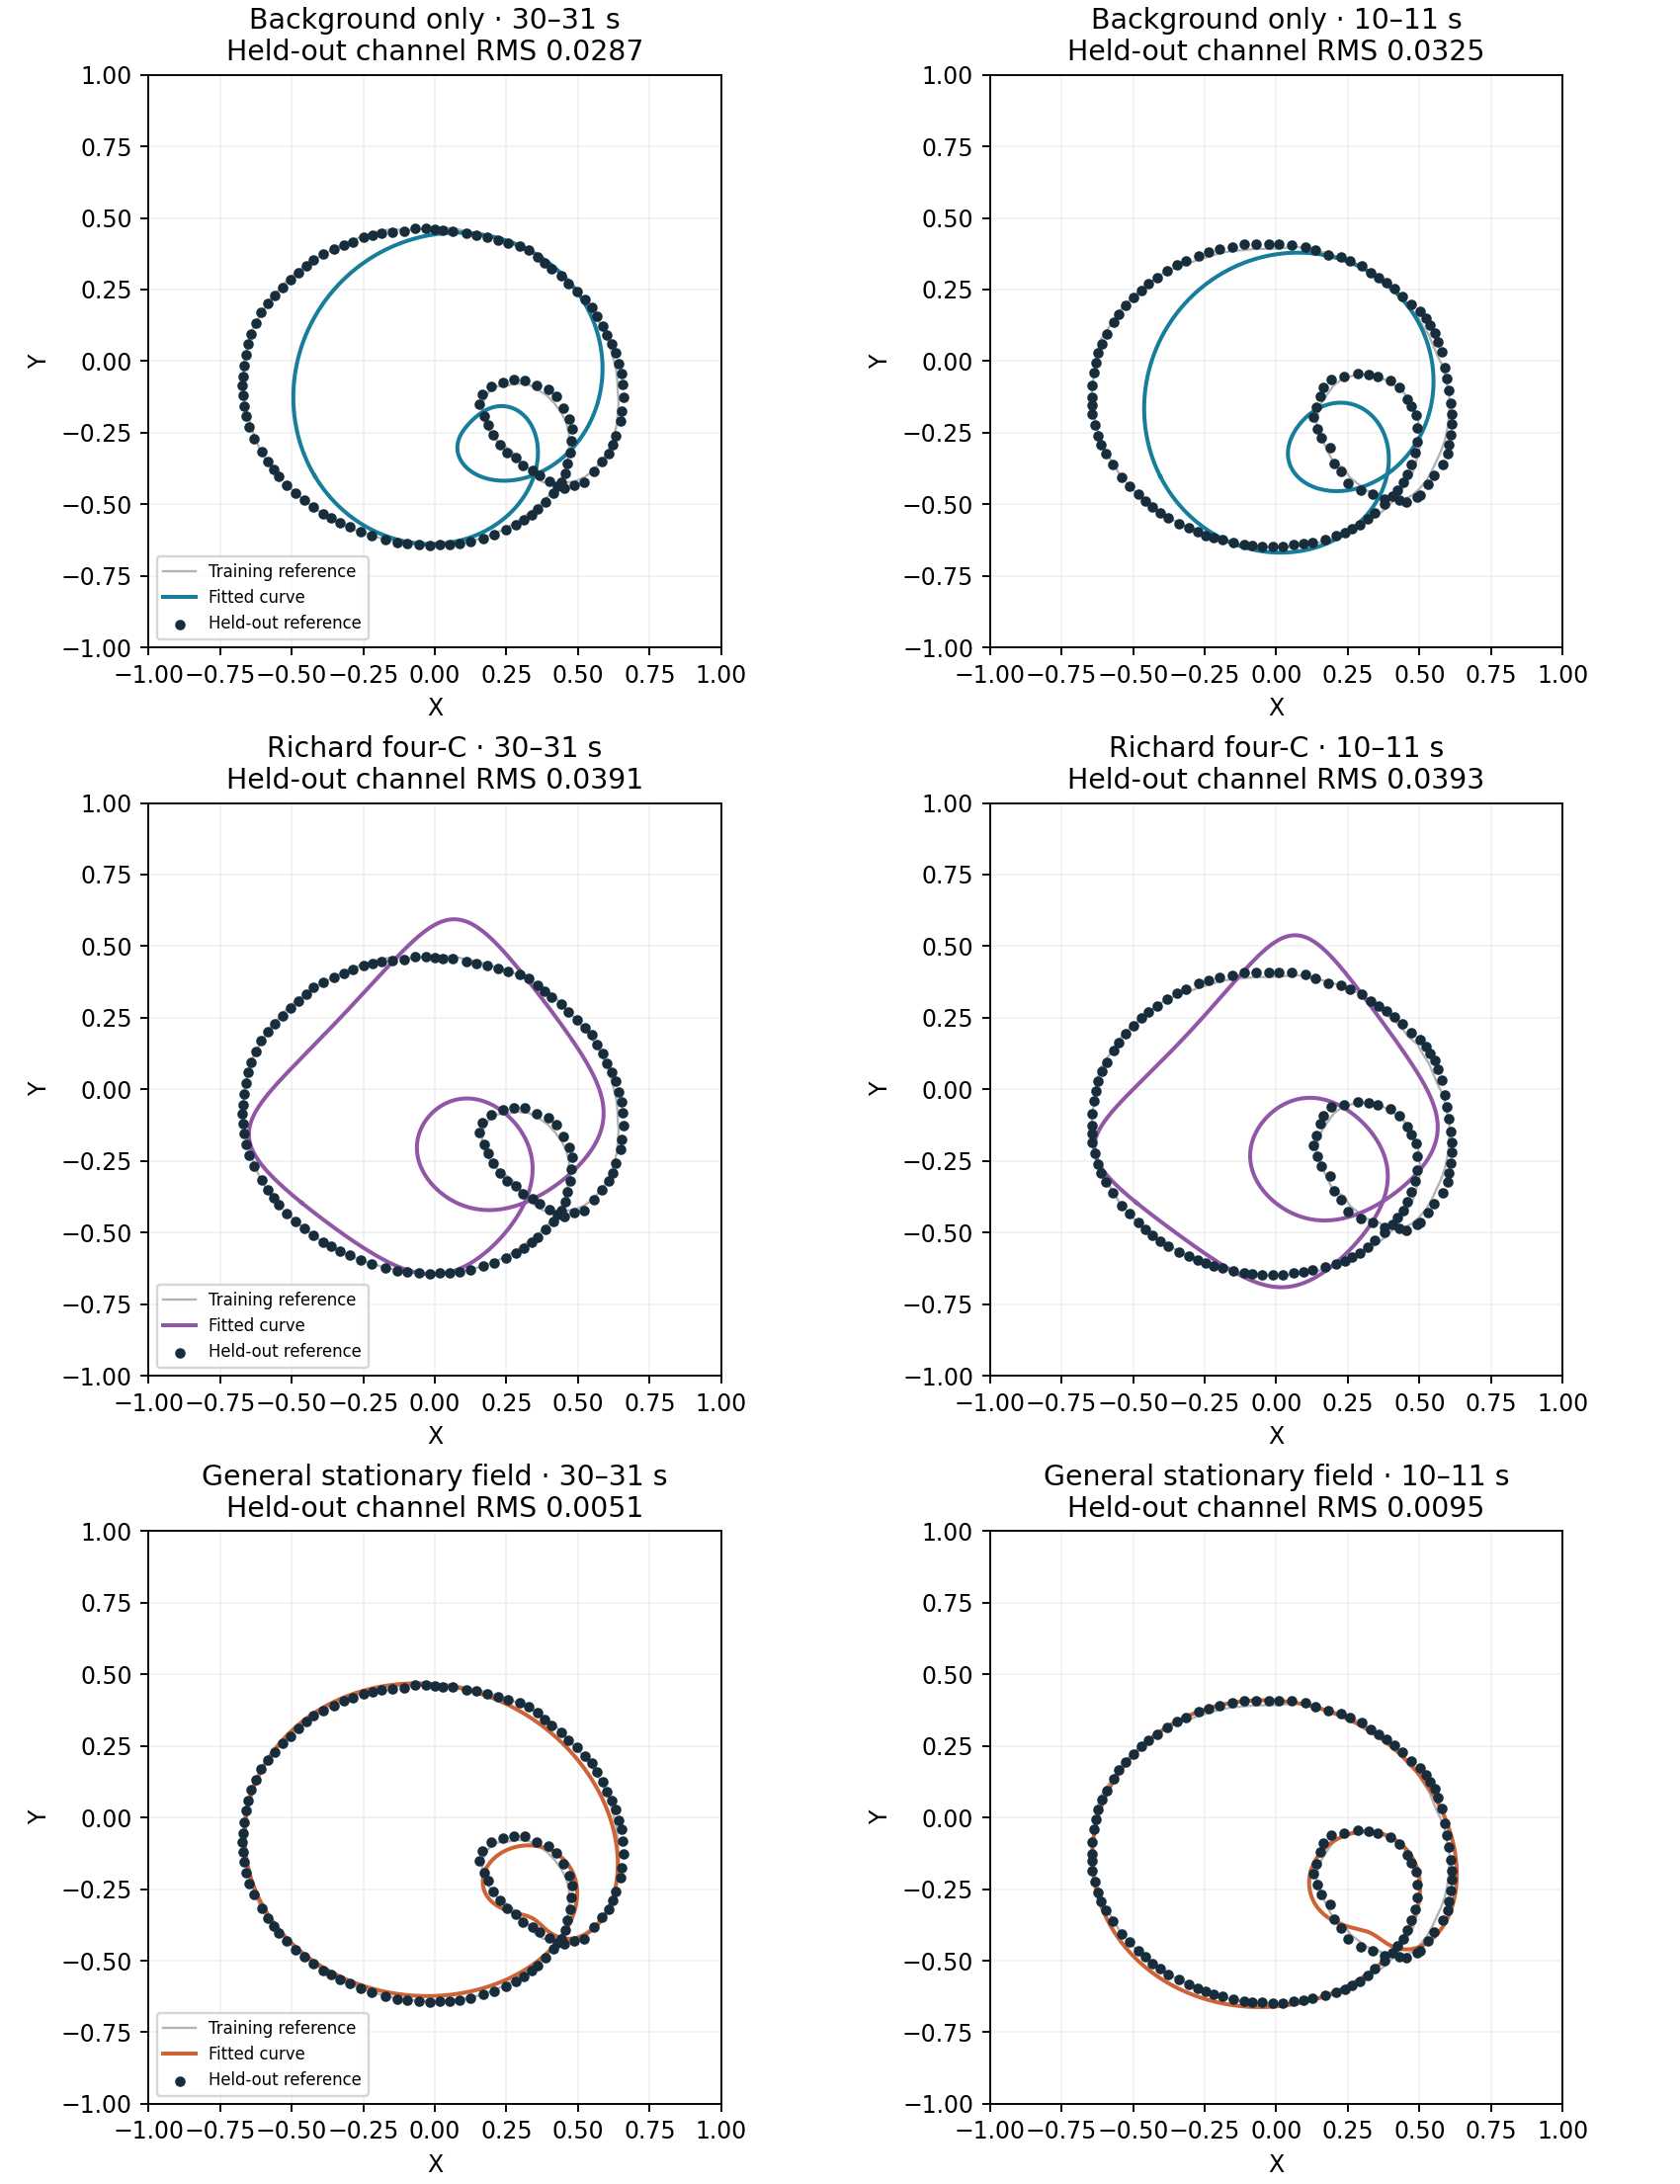
\includegraphics[width=\linewidth,height=.87\textheight,keepaspectratio]{three_models.png}
\newpage
{\Large Exactly how the reference is constructed}

1. Retain the existing complete-cycle detection and ordered channel bins. Alternate cycles form training and held-out groups: 152/152 cycles for 30--31 s, 109/108 for 10--11 s. Average corresponding four-channel bins across each group. These original 128 final-average points need not be uniformly spaced in anisotropy.

2. Join consecutive training-average \emph{four-channel vectors} by linear interpolation, including last to first. Let the resulting closed interpolant be $\mathbf I(t)$, with original bin-index coordinate $0\leq t\leq128$. Calculate ratios from interpolated channels:
\[
\mathbf a(t)=\left(\frac{I_0(t)-I_{90}(t)}{I_0(t)+I_{90}(t)},\;
\frac{I_{45}(t)-I_{135}(t)}{I_{45}(t)+I_{135}(t)}\right).
\]
3. Integrate ordered path length on a dense grid (128 subdivisions per original segment), counting both passes through any overlapping sections:
\[
s(t)=\frac{\int_0^t\|\mathbf a'(u)\|\,du}{\int_0^{128}\|\mathbf a'(u)\|\,du},\qquad
 t_j=s^{-1}(j/128),\quad j=0,\ldots,127.
\]
4. The new training reference is $\mathbf I(t_j)$. Apply exactly the same original-bin interpolation indices and weights to the held-out channel average. The held-out reference is therefore \emph{not independently made uniform}. Unequal chords also occur at high curvature even when integrated arc is uniform. This is neither direct angle inversion nor projection onto a fitted cone. Interpolation adds no independent information and correlates neighboring points.

{\Large What happens to these points in the fit?}

Freeze measured four-channel values and their order. Recompute their actual final-interpolant arc coordinates $u_j$ to handle small resampling discretization differences. For each proposed cone, brightness and background, simulate a dense full revolution of \emph{measured-model} channel intensities, including interference. Compute that predicted anisotropy's own ordered cumulative arc. Evaluate the predicted channels at
\[
s_j^{\rm model}=(\delta+\epsilon u_j)\bmod1,\qquad \epsilon\in\{-1,+1\}.
\]
There is one cyclic offset $\delta$ per window; both directions are tested. There is no independently movable point, nearest-point assignment or 16-parameter phase warp. The objective remains channel intensity:
\[
J=\sum_j\sum_{i=1}^4\left[\frac{I^{\rm pred}_{i,j}-I^{\rm train}_{i,j}}{T_j^{\rm train}}\right]^2,
\qquad T_j=\sum_i I_{i,j}.
\]
Equal bin weights approximate equal weighting along measured anisotropy arc, while division by $T_j$ retains relative-intensity weighting. This is not uniform mechanical phase, uniform angular error, or a calibrated noise likelihood. Held-out scores use frozen predictions without refitting or realignment; alternating neighboring cycles test repeatability, not independent absolute-angle truth.
\newpage
{\Large Models and results}

All models keep current gain/matrix calibration, NA 0.38--1.3, water/oil Fresnel and BFP mapping, fixed cone and one brightness $a_0$ per window. With cone direction $\mathbf d$,
\[
S_i=a_0^2\sin^2\theta\;Q_i(\mathbf d).
\]
\textbf{Background only:} $I_i=S_i+B_i$. Three background parameters set total power and independent pair contrasts, with equal pair sums, nonnegative channels, no Stokes-disk restriction. Eight fitted parameters per window: cone three, brightness one, offset one, background three.

\textbf{Richard exact four-C:}
\[
I_i=S_i+C_i\sqrt{S_i}.
\]
Four constant $C_i$ per window, no independent additive term. Nine fitted parameters per window. Numerically use $S_i=\alpha f_i$, $K_i=a_0C_i$, giving $I_i=\alpha f_i+K_i\sqrt{f_i}$. Selected $\alpha$ values are finite, but the structural $\alpha\to0$, $C_i\to\infty$ degeneracy remains possible. This empirical correction does not specify a physical background power.

\textbf{General stationary field:}
\[
I_i=\|E_{s,i}(\mathbf d)+E_{b,i}\|^2+N_i
=S_i+2\operatorname{Re}\langle E_{s,i},E_{b,i}\rangle+\|E_{b,i}\|^2+N_i.
\]
A common fixed pupil field uses ten complex transverse modes, plus a noninterfering positive-Stokes background. Field/overlap changes with orientation follow optical propagation; no freely varying per-point overlap. There are 23 shared background parameters plus five cone/brightness/offset parameters per window (33 total for both). Generality is conditional on fixed-position ideal-dipole common-pupil optics; it does not cover arbitrary source motion or independent post-analyser fields.

\begin{tabular}{llrrrr}\toprule
Window & Model & Channel RMS & XY RMS & BG/$T_{\max}$ & Folded $\theta$\\\midrule
30s & Background only & 0.0287 & 0.1098 & 35.5\% & 29.1--89.9$^\circ$ \\
30s & Richard four-C & 0.0391 & 0.1488 & --- & 29.0--88.6$^\circ$ \\
30s & General stationary field & 0.0051 & 0.0243 & 54.8\% & 6.5--89.9$^\circ$ \\
10s & Background only & 0.0325 & 0.1272 & 38.3\% & 33.7--89.9$^\circ$ \\
10s & Richard four-C & 0.0393 & 0.1570 & --- & 33.4--88.4$^\circ$ \\
10s & General stationary field & 0.0095 & 0.0419 & 54.5\% & 10.9--89.9$^\circ$ \\
\bottomrule\end{tabular}

Channel RMS is $\sqrt{\operatorname{mean}_{i,j}[(I^{pred}-I^{heldout})/T^{heldout}]^2}$, not percent error relative to each channel. XY RMS is Euclidean anisotropy error. Angles are folded to $0$--$90^\circ$ at matched reference locations. Background percentages use original training maximum total intensity; the same absolute shared field produces slightly different percentages in the two windows.

The selected stationary fit assigns essentially all represented background power to the coherent field. Its background is close to the allowed budget (54.84\% versus 55.69\% of the smaller original maximum), capped at 95\% of the stricter original minimum total intensity. This is a conditional fit composition, not a measured decomposition. A different local solution fits less closely at about 47\% background with much narrower angle ranges, emphasizing remaining identifiability concerns.

The selected stationary refinement converged. Doubling its curve resolution changes predicted intensities by less than $5\times10^{-8}T_{\max}$. Cached pupil quadrature differs from analytic unit-signal coefficients by at most $7.7\times10^{-5}$ on a test cone. Multiple starts do not certify a global optimum. The closer fit alone does not establish a unique physical field or correct recovered angles. No commit or push.
\end{document}
